\begin{center}
\begin{minipage}[h]{0.9\linewidth}
\begin{wrapfigure}{l}{0.42\textwidth}
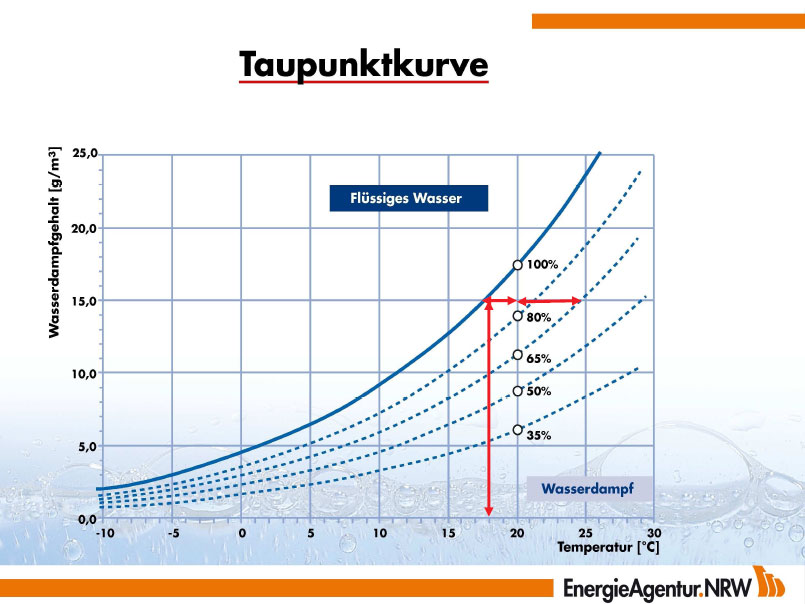
\includegraphics[width=0.42\textwidth]{graphics/Taupunktkurve.jpg}
\caption{Taupunktkurve \cite{PfefferkeineAngaben}}
\label{taupunktkurve}
\end{wrapfigure}

\NewsItem{Grundlagen der Luftfeuchtigkeitsmessung}
\vspace{3pt}

%%======================================================================== Text Einfügen
Wichtig für das allgemeine Verständnis der Feuchtemessung ist, dass es unterschiedliche Verfahren zur Messung der Feuchte gibt. Dabei befassen sich diese mit gasförmigen, flüssigen oder festen Stoffen. Hierbei geht es grundsätzlich um die Gasfeuchtemessung (\textit{Hygrometrie}). Die feuchte Luft ist demnach eine Mischung von trockener Luft und Wasserdampf, dessen Sättigungspunkt abhängig des Barometerstands und der Umgebungstemperatur ist. Bei festen Stoffen und Flüssigkeiten wird die Feuchte meistens als Wassergehalt angegeben. \cite{Hesse2014}\\[0.5cm]
Eines der Schlüsselbegriffe, auf den hier besonders eingegangen wird, ist der Taupunkt (\textit{dew point}), resp. die Taupunkttemperatur. Dabei handelt es sich um einen Punkt, bei dem die Luft mit Wasserdampf gesättigt ist (100\% Luftfeuchte). Senkt sich die Lufttemperatur unter diesen Punkt, so beginnt die Luft zu kondensieren. In der Abbildung \ref{taupunktkurve} ist das Verhältnis von Temperatur und Wasserdampfgehalt in g/m$^{3}$ graphisch dargestellt. Deutlich zu erkennen ist, wie der Wassdampfgehalt von der Temperatur abhängig ist\footnote{bei unverändertem Luftdruck}. \cite{Hesse2014}\\

\end{minipage}
\end{center}